% Created by tikzDevice version 0.12.6 on 2026-08-03 04:28:59
% !TEX encoding = UTF-8 Unicode
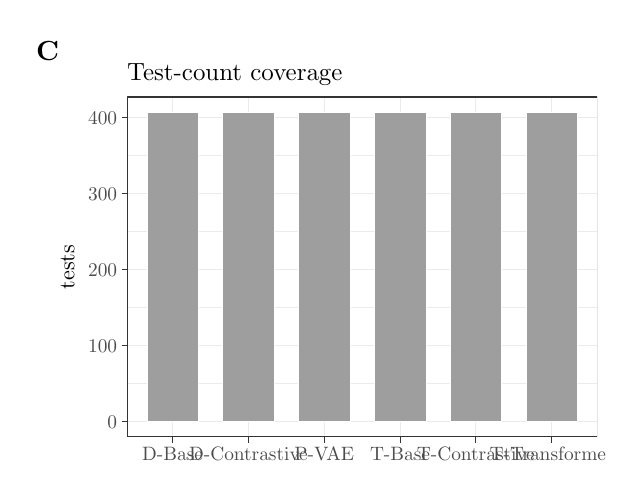
\begin{tikzpicture}[x=1pt,y=1pt]
\definecolor{fillColor}{RGB}{255,255,255}
\path[use as bounding box,fill=fillColor,fill opacity=0.00] (0,0) rectangle (208.82,161.83);
\begin{scope}
\path[clip] (  1.05,  1.74) rectangle (207.78,160.09);
\definecolor{drawColor}{RGB}{255,255,255}
\definecolor{fillColor}{RGB}{255,255,255}

\path[draw=drawColor,line width= 0.4pt,line join=round,line cap=round,fill=fillColor] (  1.05,  1.74) rectangle (207.78,160.09);
\end{scope}
\begin{scope}
\path[clip] ( 35.94, 13.93) rectangle (205.78,136.79);
\definecolor{fillColor}{RGB}{255,255,255}

\path[fill=fillColor] ( 35.94, 13.93) rectangle (205.78,136.79);
\definecolor{drawColor}{gray}{0.92}

\path[draw=drawColor,line width= 0.2pt,line join=round] ( 35.94, 33.24) --
	(205.78, 33.24);

\path[draw=drawColor,line width= 0.2pt,line join=round] ( 35.94, 60.68) --
	(205.78, 60.68);

\path[draw=drawColor,line width= 0.2pt,line join=round] ( 35.94, 88.12) --
	(205.78, 88.12);

\path[draw=drawColor,line width= 0.2pt,line join=round] ( 35.94,115.57) --
	(205.78,115.57);

\path[draw=drawColor,line width= 0.4pt,line join=round] ( 35.94, 19.52) --
	(205.78, 19.52);

\path[draw=drawColor,line width= 0.4pt,line join=round] ( 35.94, 46.96) --
	(205.78, 46.96);

\path[draw=drawColor,line width= 0.4pt,line join=round] ( 35.94, 74.40) --
	(205.78, 74.40);

\path[draw=drawColor,line width= 0.4pt,line join=round] ( 35.94,101.84) --
	(205.78,101.84);

\path[draw=drawColor,line width= 0.4pt,line join=round] ( 35.94,129.29) --
	(205.78,129.29);

\path[draw=drawColor,line width= 0.4pt,line join=round] ( 52.38, 13.93) --
	( 52.38,136.79);

\path[draw=drawColor,line width= 0.4pt,line join=round] ( 79.77, 13.93) --
	( 79.77,136.79);

\path[draw=drawColor,line width= 0.4pt,line join=round] (107.17, 13.93) --
	(107.17,136.79);

\path[draw=drawColor,line width= 0.4pt,line join=round] (134.56, 13.93) --
	(134.56,136.79);

\path[draw=drawColor,line width= 0.4pt,line join=round] (161.95, 13.93) --
	(161.95,136.79);

\path[draw=drawColor,line width= 0.4pt,line join=round] (189.34, 13.93) --
	(189.34,136.79);
\definecolor{drawColor}{RGB}{255,255,255}
\definecolor{fillColor}{gray}{0.62}

\path[draw=drawColor,line width= 0.2pt,fill=fillColor] (152.64, 19.52) rectangle (171.26,131.21);

\path[draw=drawColor,line width= 0.2pt,fill=fillColor] (180.03, 19.52) rectangle (198.66,131.21);

\path[draw=drawColor,line width= 0.2pt,fill=fillColor] (125.24, 19.52) rectangle (143.87,131.21);

\path[draw=drawColor,line width= 0.2pt,fill=fillColor] ( 70.46, 19.52) rectangle ( 89.09,131.21);

\path[draw=drawColor,line width= 0.2pt,fill=fillColor] ( 97.85, 19.52) rectangle (116.48,131.21);

\path[draw=drawColor,line width= 0.2pt,fill=fillColor] ( 43.07, 19.52) rectangle ( 61.69,131.21);
\definecolor{drawColor}{gray}{0.20}

\path[draw=drawColor,line width= 0.4pt,line join=round,line cap=round] ( 35.94, 13.93) rectangle (205.78,136.79);
\end{scope}
\begin{scope}
\path[clip] (  0.00,  0.00) rectangle (208.82,161.83);
\definecolor{drawColor}{gray}{0.30}

\node[text=drawColor,anchor=base east,inner sep=0pt, outer sep=0pt, scale=  0.70] at ( 32.34, 17.11) {0};

\node[text=drawColor,anchor=base east,inner sep=0pt, outer sep=0pt, scale=  0.70] at ( 32.34, 44.55) {100};

\node[text=drawColor,anchor=base east,inner sep=0pt, outer sep=0pt, scale=  0.70] at ( 32.34, 71.99) {200};

\node[text=drawColor,anchor=base east,inner sep=0pt, outer sep=0pt, scale=  0.70] at ( 32.34, 99.43) {300};

\node[text=drawColor,anchor=base east,inner sep=0pt, outer sep=0pt, scale=  0.70] at ( 32.34,126.88) {400};
\end{scope}
\begin{scope}
\path[clip] (  0.00,  0.00) rectangle (208.82,161.83);
\definecolor{drawColor}{gray}{0.20}

\path[draw=drawColor,line width= 0.4pt,line join=round] ( 33.94, 19.52) --
	( 35.94, 19.52);

\path[draw=drawColor,line width= 0.4pt,line join=round] ( 33.94, 46.96) --
	( 35.94, 46.96);

\path[draw=drawColor,line width= 0.4pt,line join=round] ( 33.94, 74.40) --
	( 35.94, 74.40);

\path[draw=drawColor,line width= 0.4pt,line join=round] ( 33.94,101.84) --
	( 35.94,101.84);

\path[draw=drawColor,line width= 0.4pt,line join=round] ( 33.94,129.29) --
	( 35.94,129.29);
\end{scope}
\begin{scope}
\path[clip] (  0.00,  0.00) rectangle (208.82,161.83);
\definecolor{drawColor}{gray}{0.20}

\path[draw=drawColor,line width= 0.4pt,line join=round] ( 52.38, 11.93) --
	( 52.38, 13.93);

\path[draw=drawColor,line width= 0.4pt,line join=round] ( 79.77, 11.93) --
	( 79.77, 13.93);

\path[draw=drawColor,line width= 0.4pt,line join=round] (107.17, 11.93) --
	(107.17, 13.93);

\path[draw=drawColor,line width= 0.4pt,line join=round] (134.56, 11.93) --
	(134.56, 13.93);

\path[draw=drawColor,line width= 0.4pt,line join=round] (161.95, 11.93) --
	(161.95, 13.93);

\path[draw=drawColor,line width= 0.4pt,line join=round] (189.34, 11.93) --
	(189.34, 13.93);
\end{scope}
\begin{scope}
\path[clip] (  0.00,  0.00) rectangle (208.82,161.83);
\definecolor{drawColor}{gray}{0.30}

\node[text=drawColor,anchor=base,inner sep=0pt, outer sep=0pt, scale=  0.70] at ( 52.38,  5.51) {D-Base};

\node[text=drawColor,anchor=base,inner sep=0pt, outer sep=0pt, scale=  0.70] at ( 79.77,  5.51) {D-Contrastive};

\node[text=drawColor,anchor=base,inner sep=0pt, outer sep=0pt, scale=  0.70] at (107.17,  5.51) {P-VAE};

\node[text=drawColor,anchor=base,inner sep=0pt, outer sep=0pt, scale=  0.70] at (134.56,  5.51) {T-Base};

\node[text=drawColor,anchor=base,inner sep=0pt, outer sep=0pt, scale=  0.70] at (161.95,  5.51) {T-Contrastive};

\node[text=drawColor,anchor=base,inner sep=0pt, outer sep=0pt, scale=  0.70] at (189.34,  5.51) {T-Transformer};
\end{scope}
\begin{scope}
\path[clip] (  0.00,  0.00) rectangle (208.82,161.83);
\definecolor{drawColor}{RGB}{0,0,0}

\node[text=drawColor,rotate= 90.00,anchor=base,inner sep=0pt, outer sep=0pt, scale=  0.80] at ( 16.86, 75.36) {tests};
\end{scope}
\begin{scope}
\path[clip] (  0.00,  0.00) rectangle (208.82,161.83);
\definecolor{drawColor}{RGB}{0,0,0}

\node[text=drawColor,anchor=base west,inner sep=0pt, outer sep=0pt, scale=  0.90] at ( 35.94,142.78) {Test-count coverage};
\end{scope}
\begin{scope}
\path[clip] (  0.00,  0.00) rectangle (208.82,161.83);
\definecolor{drawColor}{RGB}{0,0,0}

\node[text=drawColor,anchor=base,inner sep=0pt, outer sep=0pt, scale=  1.00] at (  7.20,150.08) {\bfseries C};
\end{scope}
\end{tikzpicture}
